\documentclass[11pt,a4paper]{report}
\usepackage[textwidth=37em,vmargin=30mm]{geometry}
\usepackage{calc,xunicode,amsmath,amssymb,paralist,enumitem,tabu,booktabs,datetime2,xeCJK,xeCJKfntef,listings}
\usepackage{tocloft,fancyhdr,tcolorbox,xcolor,graphicx,eso-pic,xltxtra,xelatexemoji}

\newcommand{\envyear}[0]{2025}
\newcommand{\envdatestr}[0]{2025-02-17}
\newcommand{\envfinaldir}[0]{webdb/2025/20250217/final}

\usepackage[hidelinks]{hyperref}
\hypersetup{
    colorlinks=false,
    pdfpagemode=FullScreen,
    pdftitle={Web Digest - \envdatestr}
}

\setlength{\cftbeforechapskip}{10pt}
\renewcommand{\cftchapfont}{\rmfamily\bfseries\large\raggedright}
\setlength{\cftbeforesecskip}{2pt}
\renewcommand{\cftsecfont}{\sffamily\small\raggedright}

\setdefaultleftmargin{2em}{2em}{1em}{1em}{1em}{1em}

\usepackage{xeCJK,xeCJKfntef}
\xeCJKsetup{PunctStyle=plain,RubberPunctSkip=false,CJKglue=\strut\hskip 0pt plus 0.1em minus 0.05em,CJKecglue=\strut\hskip 0.22em plus 0.2em}
\XeTeXlinebreaklocale "zh"
\XeTeXlinebreakskip = 0pt


\setmainfont{Brygada 1918}
\setromanfont{Brygada 1918}
\setsansfont{IBM Plex Sans}
\setmonofont{JetBrains Mono NL}
\setCJKmainfont{Noto Serif CJK SC}
\setCJKromanfont{Noto Serif CJK SC}
\setCJKsansfont{Noto Sans CJK SC}
\setCJKmonofont{Noto Sans CJK SC}

\setlength{\parindent}{0pt}
\setlength{\parskip}{8pt}
\linespread{1.15}

\lstset{
	basicstyle=\ttfamily\footnotesize,
	numbersep=5pt,
	backgroundcolor=\color{black!5},
	showspaces=false,
	showstringspaces=false,
	showtabs=false,
	tabsize=2,
	captionpos=b,
	breaklines=true,
	breakatwhitespace=true,
	breakautoindent=true,
	linewidth=\textwidth
}






\newcommand{\coverpic}[2]{
    % argv: itemurl, authorname
    Cover photo by #2~~(\href{#1}{#1})
}
\newcommand{\makeheader}[0]{
    \begin{titlepage}
        % \newgeometry{hmargin=15mm,tmargin=21mm,bmargin=12mm}
        \begin{center}
            
            \rmfamily\scshape
            \fontspec{BaskervilleF}
            \fontspec{Old Standard}
            \fontsize{59pt}{70pt}\selectfont
            WEB\hfill DIGEST
            
            \vfill
            % \vskip 30pt
            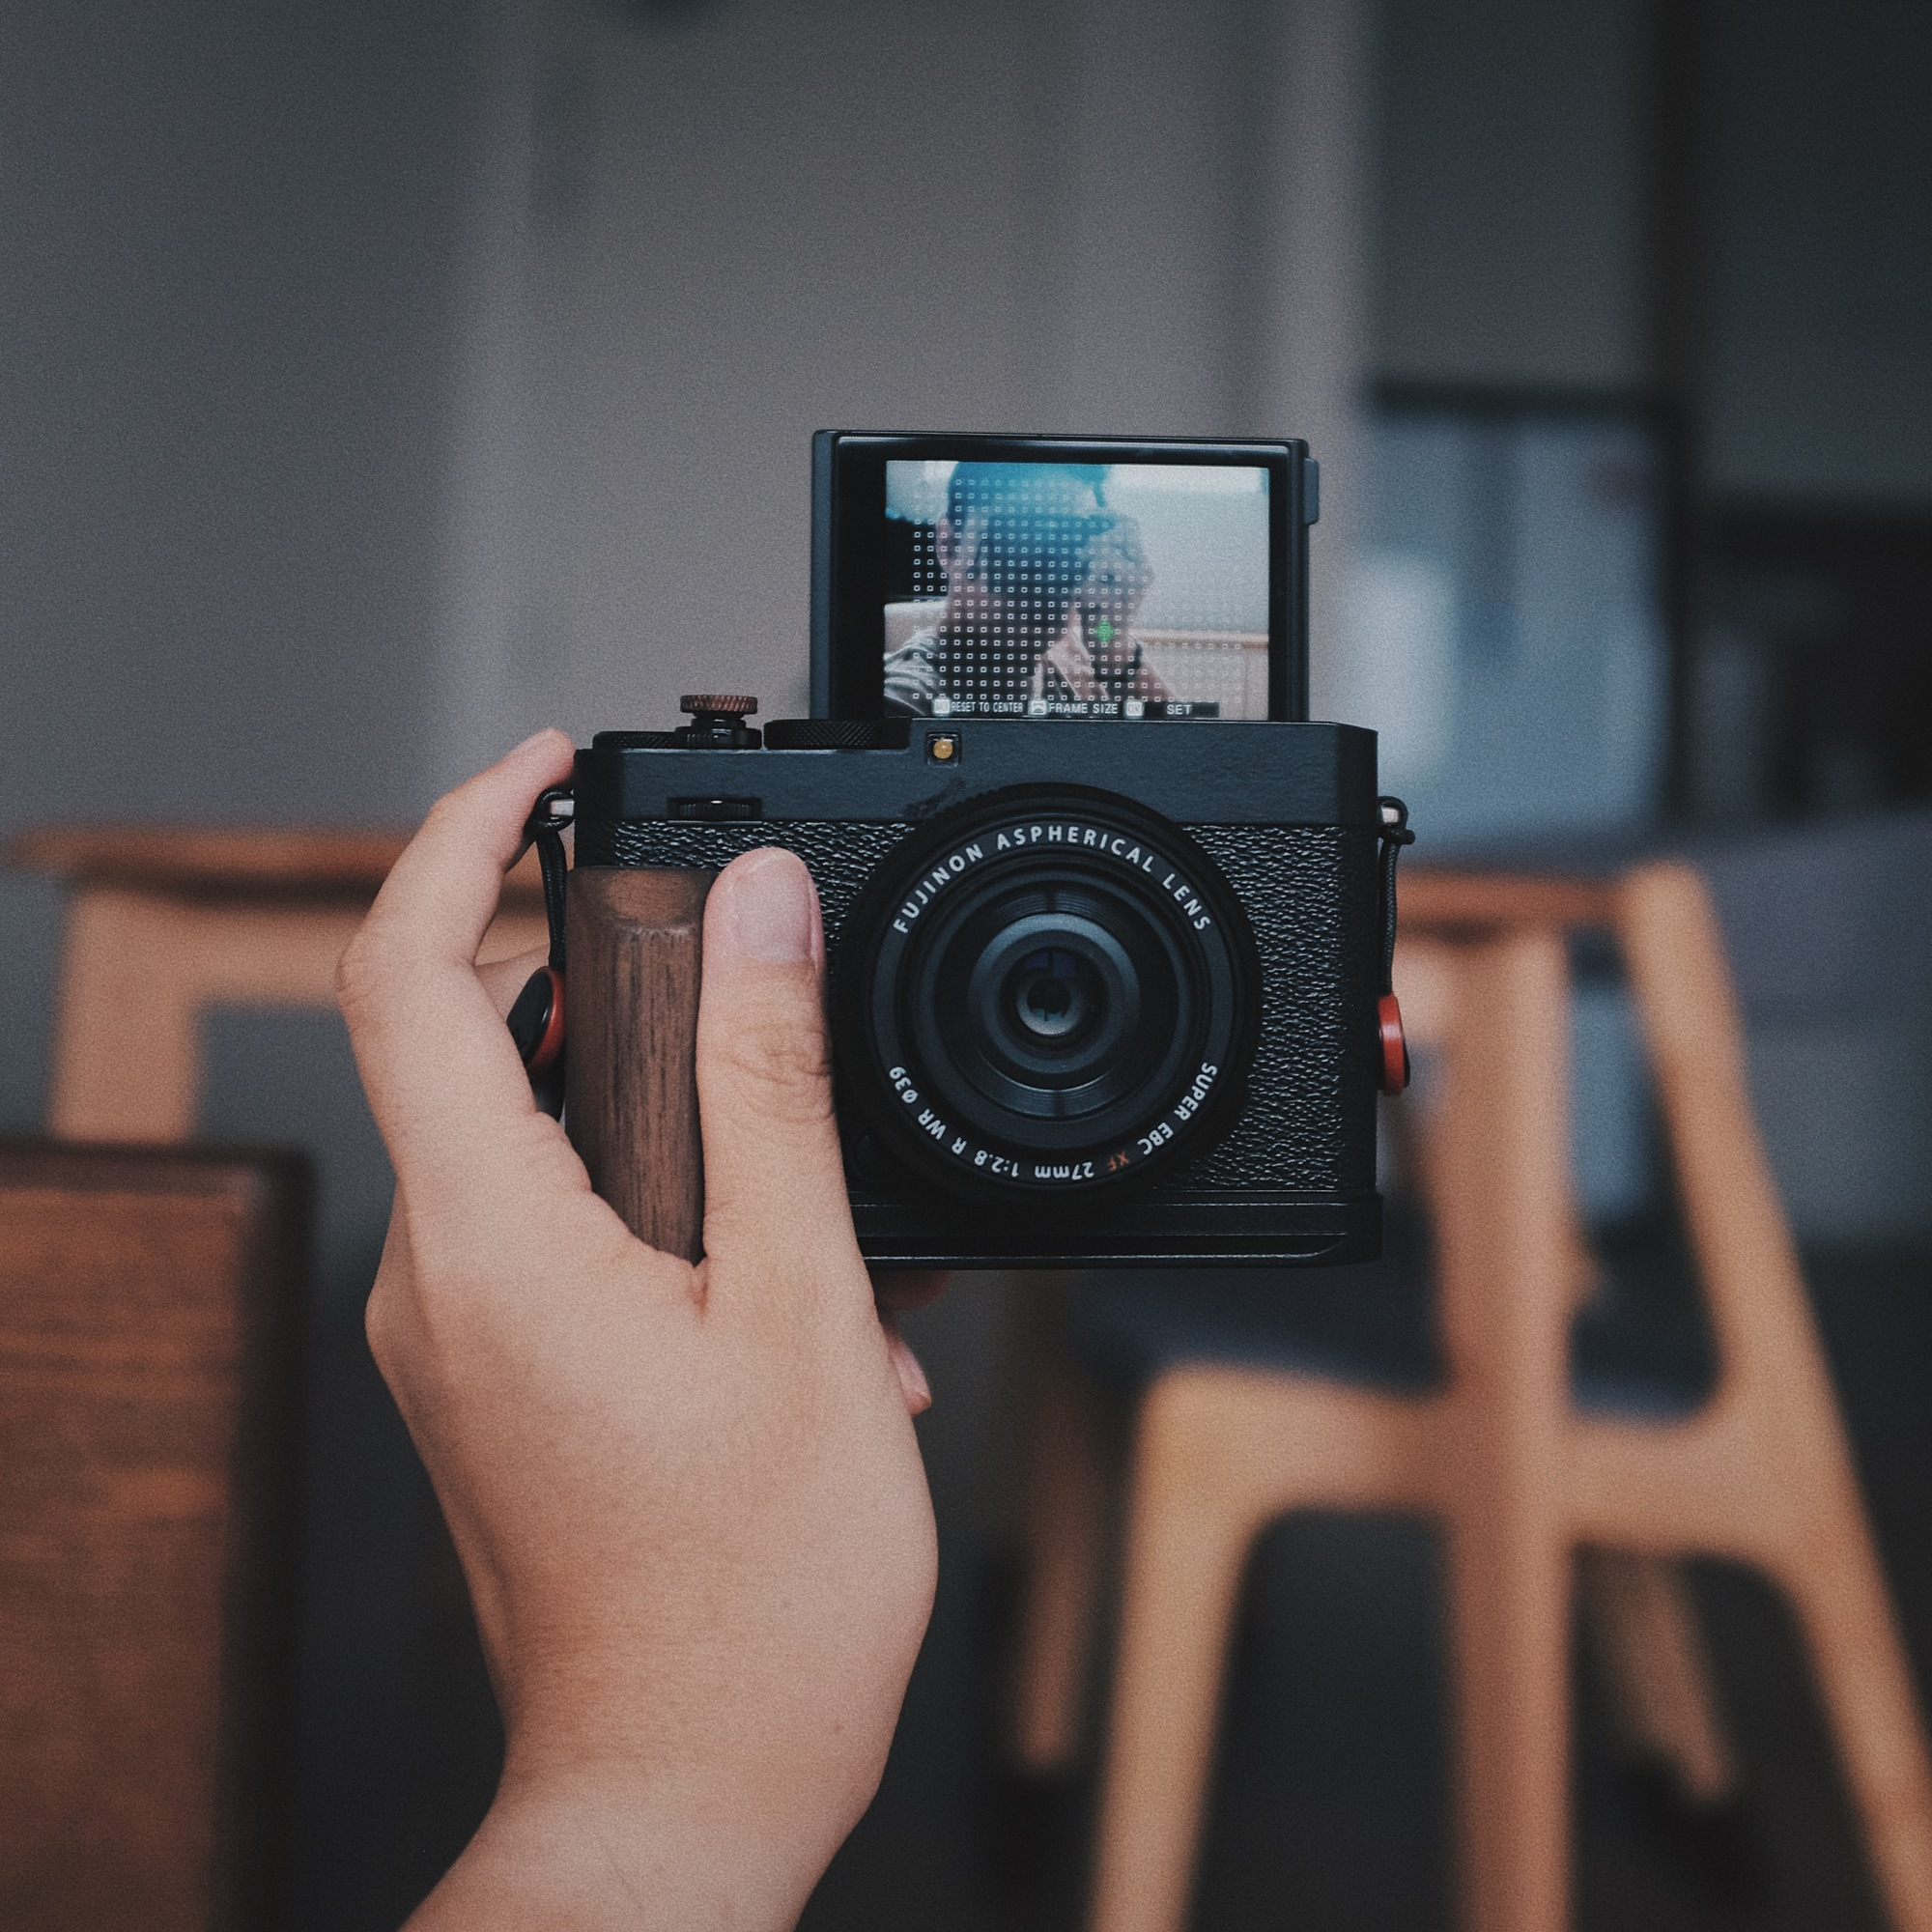
\includegraphics[width=\linewidth]{\envfinaldir/coverpic-prod.jpg}\par
            % \vskip 30pt
            \vfill

            \normalsize\rmfamily\scshape
            \copyright{} The Web Digest Project \hfill\large \envdatestr
        \end{center}
    \end{titlepage}
    % \restoregeometry
}
\newcommand{\simplehref}[1]{%
    \textcolor{blue!80!green}{\href{#1}{#1}}%
}
\renewcommand{\contentsname}{\center\Huge\sffamily\bfseries Contents\par\vskip 20pt}
\newcounter{ipartcounter}
\setcounter{ipartcounter}{0}
\newcommand{\ipart}[1]{
    % \vskip 20pt
    \clearpage
    \stepcounter{ipartcounter}
    \phantomsection
    \addcontentsline{toc}{chapter}{#1}
    % \begin{center}
    %     \Huge
    %     \sffamily\bfseries
    %     #1
    % \end{center}
    % \vskip 20pt plus 7pt
}
\newcounter{ichaptercounter}
\setcounter{ichaptercounter}{0}
\newcommand{\ichapter}[1]{
    % \vskip 20pt
    \clearpage
    \stepcounter{ichaptercounter}
    \phantomsection
    \addcontentsline{toc}{section}{\numberline{\arabic{ichaptercounter}}#1}
    \begin{center}
        \Huge
        \sffamily\bfseries
        #1
    \end{center}
    \vskip 20pt plus 7pt
}
\newcommand{\entrytitlefont}[1]{\subsection*{\raggedright\Large\sffamily\bfseries#1}}
\newcommand{\entryitemGeneric}[2]{
    % argv: title, url
    \parbox{\linewidth}{
        \entrytitlefont{#1}\par\vskip 5pt
        \footnotesize\ttfamily\mdseries
        \simplehref{#2}
    }\vskip 11pt plus 11pt minus 1pt
}
\newcommand{\entryitemGithub}[3]{
    % argv: title, url, desc
    \parbox{\linewidth}{
        \entrytitlefont{#1}\par\vskip 5pt
        \footnotesize\ttfamily\mdseries
        \simplehref{#2}\par\vskip 5pt
        \small\rmfamily\mdseries#3
    }\vskip 11pt plus 11pt minus 1pt
}
\newcommand{\entryitemAp}[3]{
    % argv: title, url, desc
    \parbox{\linewidth}{
        \entrytitlefont{#1}\par\vskip 5pt
        \footnotesize\ttfamily\mdseries
        \simplehref{#2}\par\vskip 5pt
        \small\rmfamily\mdseries#3
    }\vskip 11pt plus 11pt minus 1pt
}
\newcommand{\entryitemHackernews}[3]{
    % argv: title, hnurl, rawurl
    % \parbox{\linewidth}{
    %     \entrytitlefont{#1}\par\vskip 5pt
    %     \footnotesize\ttfamily\mdseries
    %     \simplehref{#3}\par
    %     \textcolor{black!50}{\href{#2}{#2}}
    % }\vskip 11pt plus 11pt minus 1pt
    \begin{minipage}{\linewidth}
            \entrytitlefont{#1}\par\vskip 5pt
            \footnotesize\ttfamily\mdseries
            \simplehref{#3}\par
            \textcolor{black!50}{\href{#2}{#2}}
    \end{minipage}\par\vskip 11pt plus 11pt minus 1pt
}







\begin{document}

\makeheader

\tableofcontents\clearpage




\ipart{Developers}
\ichapter{Hacker News}
\entryitemTwoLinks{Big tech has disrupted the social contract}{https://news.ycombinator.com/item?id=43071213}{https://basedfob.substack.com/p/big-tech-has-disrupted-the-social}

\entryitemTwoLinks{Kindle is removing download and transfer option on Feb 26th}{https://news.ycombinator.com/item?id=43070155}{https://old.reddit.com/r/kindle/comments/1inr9uy/fyi\_amazon\_is\_removing\_download\_transfer\_option/}

\entryitemTwoLinks{Caddy – The Ultimate Server with Automatic HTTPS}{https://news.ycombinator.com/item?id=43070025}{https://caddyserver.com/}

\entryitemTwoLinks{Half-Life 2 and Dishonored art lead Viktor Antonov has died}{https://news.ycombinator.com/item?id=43069514}{https://www.eurogamer.net/half-life-2-and-dishonored-art-lead-viktor-antonov-dies-aged-just-52}

\entryitemTwoLinks{United States Power Outage Map}{https://news.ycombinator.com/item?id=43069399}{https://poweroutage.us/}

\entryitemTwoLinks{Vim after Bram: a core maintainer on how they've kept it going}{https://news.ycombinator.com/item?id=43068884}{https://thenewstack.io/vim-after-bram-a-core-maintainer-on-how-theyve-kept-it-going/}

\entryitemTwoLinks{Flea-Scope: \$18 Source Available USB Oscilloscope, Logic Analyzer and More [pdf]}{https://news.ycombinator.com/item?id=43068585}{https://rtestardi.github.io/usbte/flea-scope.pdf}

\entryitemTwoLinks{Rust Is Eating JavaScript (2023)}{https://news.ycombinator.com/item?id=43067585}{https://leerob.com/n/rust}

\entryitemTwoLinks{Finding Flow: Escaping digital distractions through deep work and slow living}{https://news.ycombinator.com/item?id=43067303}{https://www.ssp.sh/blog/finding-flow/}

\entryitemTwoLinks{``A calculator app? Anyone could make that''}{https://news.ycombinator.com/item?id=43066953}{https://chadnauseam.com/coding/random/calculator-app}

\entryitemTwoLinks{50 Years of Travel Tips}{https://news.ycombinator.com/item?id=43066720}{https://kk.org/thetechnium/50-years-of-travel-tips/}

\entryitemTwoLinks{US government struggles to rehire nuclear safety staff it laid off days ago}{https://news.ycombinator.com/item?id=43066182}{https://www.bbc.com/news/articles/c4g3nrx1dq5o}

\entryitemTwoLinks{Dinner at a North Korean Restaurant in Shanghai (2016)}{https://news.ycombinator.com/item?id=43065586}{https://simplyfabulicious.wordpress.com/2016/09/09/dinner-at-a-north-korean-restaurant-in-shanghai/}

\entryitemTwoLinks{Gixy: Nginx Configuration Static Analyzer}{https://news.ycombinator.com/item?id=43065217}{https://github.com/dvershinin/gixy}

\entryitemTwoLinks{How Medical Research Cuts Would Hit Colleges and Hospitals in Every State}{https://news.ycombinator.com/item?id=43064637}{https://www.nytimes.com/interactive/2025/02/13/upshot/nih-trump-funding-cuts.html}

\entryitemTwoLinks{US Forest Service and National Park Service to fire thousands of workers}{https://news.ycombinator.com/item?id=43064466}{https://www.theguardian.com/us-news/2025/feb/15/us-forest-service-national-park-service-layoffs}

\entryitemTwoLinks{The Sims Game Design Documents (1997)}{https://news.ycombinator.com/item?id=43064273}{https://donhopkins.com/home/TheSimsDesignDocuments/}

\entryitemTwoLinks{Show HN: Blunderchess.net – blunder for your opponent every five moves}{https://news.ycombinator.com/item?id=43063970}{https://blunderchess.net}

\entryitemTwoLinks{Jellyfin: The Free Software Media System}{https://news.ycombinator.com/item?id=43063167}{https://jellyfin.org/}

\entryitemTwoLinks{Watt The Fox?}{https://news.ycombinator.com/item?id=43062546}{https://h.43z.one/blog/2025-02-12/}\ichapter{Phoronix}
\entryitemGeneric{\hskip 0pt{}Linux 6.14-rc3 Released With Faux Bus \& Various Fixes}{https://www.phoronix.com/news/Linux-6.14-rc3-Released}

\entryitemGeneric{\hskip 0pt{}New "Faux Bus" API Merged For Linux 6.14 - Including Both Rust \& C Bindings}{https://www.phoronix.com/news/Linux-6.14-Faux-Bus-Merged}

\entryitemGeneric{\hskip 0pt{}Firefox User Manages Experimental Browser Port To GTK4 Toolkit}{https://www.phoronix.com/news/Firefox-User-Ports-GTK4}

\entryitemGeneric{\hskip 0pt{}GNOME 48 Beta Released With HDR Bits, gdctl, Adwaita Fonts Default \& More}{https://www.phoronix.com/news/GNOME-48-Beta-Released}

\entryitemGeneric{\hskip 0pt{}Intel Killer E5000 Ethernet Support For Linux 6.15}{https://www.phoronix.com/news/Intel-Killer-E5000-Linux-6.15}

\entryitemGeneric{\hskip 0pt{}Btrfs-Progs 6.13 Released With "mkfs.btrfs --compress" Support}{https://www.phoronix.com/news/Btrfs-Progs-6.13}

\entryitemGeneric{\hskip 0pt{}134k Lines Of Code Posted As Latest Effort For COBOL Support Within GCC}{https://www.phoronix.com/news/134k-Lines-v2-COBOL-For-GCC}

\entryitemGeneric{\hskip 0pt{}FreeBSD 13.5 Overcomes UFS Y2038 Problem To Push It Out To Year 2106}{https://www.phoronix.com/news/FreeBSD-13.5-Beta-2}

\entryitemGeneric{\hskip 0pt{}NTSYNC Driver Fix Being Worked On For Proper User Permissions}{https://www.phoronix.com/news/Linux-NTSYNC-Permissions-Issue}\ichapter{Dribbble}
\entryitemGeneric{\hskip 0pt{}Alpaca}{https://dribbble.com/shots/25627851-Alpaca}

\entryitemGeneric{\hskip 0pt{}Oh Baby!!}{https://dribbble.com/shots/25630659-Oh-Baby}

\entryitemGeneric{\hskip 0pt{}Ethereum Wordmark Logo Concept}{https://dribbble.com/shots/25623390-Ethereum-Wordmark-Logo-Concept}

\entryitemGeneric{\hskip 0pt{}Illustration}{https://dribbble.com/shots/25619766-Illustration}

\entryitemGeneric{\hskip 0pt{}Carbon Solutions B2B Dashboard Design}{https://dribbble.com/shots/25554521-Carbon-Solutions-B2B-Dashboard-Design}

\entryitemGeneric{\hskip 0pt{}Love Potion}{https://dribbble.com/shots/25619714-Love-Potion}

\entryitemGeneric{\hskip 0pt{}Mortar\&Carrot}{https://dribbble.com/shots/25619708-Mortar-Carrot}

\entryitemGeneric{\hskip 0pt{}Pirate Parrot}{https://dribbble.com/shots/25619077-Pirate-Parrot}

\entryitemGeneric{\hskip 0pt{}SPROXX - LOGO DESIGN}{https://dribbble.com/shots/25619328-SPROXX-LOGO-DESIGN}

\entryitemGeneric{\hskip 0pt{}Master / God / Cloud}{https://dribbble.com/shots/25619810-Master-God-Cloud}

\entryitemGeneric{\hskip 0pt{}Fast Turn Fittings}{https://dribbble.com/shots/25619395-Fast-Turn-Fittings}

\entryitemGeneric{\hskip 0pt{}Black Cat Speed Shop®}{https://dribbble.com/shots/25614666-Black-Cat-Speed-Shop}

\entryitemGeneric{\hskip 0pt{}Fintech icons pack download}{https://dribbble.com/shots/25607159-Fintech-icons-pack-download}

\entryitemGeneric{\hskip 0pt{}Self Love}{https://dribbble.com/shots/25607914-Self-Love}

\entryitemGeneric{\hskip 0pt{}Urban Echo}{https://dribbble.com/shots/25608526-Urban-Echo}

\entryitemGeneric{\hskip 0pt{}Cloaked Wireless Device}{https://dribbble.com/shots/25403560-Cloaked-Wireless-Device}

\entryitemGeneric{\hskip 0pt{}Logo tip 001. Symmetry and asymmetry}{https://dribbble.com/shots/25606111-Logo-tip-001-Symmetry-and-asymmetry}

\entryitemGeneric{\hskip 0pt{}World Peace}{https://dribbble.com/shots/25609765-World-Peace}

\entryitemGeneric{\hskip 0pt{}Sentinal - Logo Design}{https://dribbble.com/shots/25606497-Sentinal-Logo-Design}

\entryitemGeneric{\hskip 0pt{}Tanuki}{https://dribbble.com/shots/25606258-Tanuki}

\entryitemGeneric{\hskip 0pt{}Dirty Dutch - Brand Mark / Logo}{https://dribbble.com/shots/25604523-Dirty-Dutch-Brand-Mark-Logo}

\entryitemGeneric{\hskip 0pt{}Cast AI Logo Redesign}{https://dribbble.com/shots/25607135-Cast-AI-Logo-Redesign}

\entryitemGeneric{\hskip 0pt{}Running Partners}{https://dribbble.com/shots/25606250-Running-Partners}

\entryitemGeneric{\hskip 0pt{}Android Dynamic Island}{https://dribbble.com/shots/25604942-Android-Dynamic-Island}


\ipart{Developers~~~~(zh-Hans)}
\ichapter{Solidot}
\entryitemGeneric{\hskip 0pt{}窃取机密的黑客兼职勒索软件攻击者}{https://www.solidot.org/story?sid=80569}

\entryitemGeneric{\hskip 0pt{}世界海冰面积再创新低}{https://www.solidot.org/story?sid=80568}

\entryitemGeneric{\hskip 0pt{}Meta 将建造世界最长的海底光缆}{https://www.solidot.org/story?sid=80567}

\entryitemGeneric{\hskip 0pt{}大肠杆菌在死亡后会自行分解以帮助邻近细胞}{https://www.solidot.org/story?sid=80566}

\entryitemGeneric{\hskip 0pt{}Square Enix 以无法修复的 bug 为由关闭 iOS 版本的《最终幻想水晶编年史》}{https://www.solidot.org/story?sid=80565}

\entryitemGeneric{\hskip 0pt{}亚马逊将关闭 Kindle 的 Download \& Transfer via USB 功能}{https://www.solidot.org/story?sid=80564}

\entryitemGeneric{\hskip 0pt{}摩根大通 CEO 对反对重返办公室的意见不屑一顾}{https://www.solidot.org/story?sid=80563}

\entryitemGeneric{\hskip 0pt{}20 光年外的一颗恒星宜居带有行星}{https://www.solidot.org/story?sid=80562}

\entryitemGeneric{\hskip 0pt{}美摄起诉字节跳动抄袭代码获赔 8266.8 万元}{https://www.solidot.org/story?sid=80561}

\entryitemGeneric{\hskip 0pt{}俄罗斯无人机攻击切尔诺贝利核电站}{https://www.solidot.org/story?sid=80560}

\entryitemGeneric{\hskip 0pt{}Zed 使用开源模型 Zeta 预测用户的编辑}{https://www.solidot.org/story?sid=80559}

\entryitemGeneric{\hskip 0pt{}Arm 将自己制造芯片}{https://www.solidot.org/story?sid=80558}

\entryitemGeneric{\hskip 0pt{}作为换囚交易的一部分美国释放了 BTC-e 联合创始人}{https://www.solidot.org/story?sid=80557}

\entryitemGeneric{\hskip 0pt{}攻读博士学位的人数在减少}{https://www.solidot.org/story?sid=80556}

\entryitemGeneric{\hskip 0pt{}中国居民对 AI 的信任高于美国}{https://www.solidot.org/story?sid=80555}

\entryitemGeneric{\hskip 0pt{}研究发现 AI 的新闻摘要会经常性的扭曲事实}{https://www.solidot.org/story?sid=80554}

\entryitemGeneric{\hskip 0pt{}Google 和苹果恢复上架 TikTok}{https://www.solidot.org/story?sid=80553}\ichapter{V2EX}
\entryitemGeneric{\hskip 0pt{}[分享发现] 万斯在慕尼黑发言 (演讲概要+核心观点)}{https://www.v2ex.com/t/1111864}

\entryitemGeneric{\hskip 0pt{}[Apple] 国补 macbookair m3 24g 512g 6999}{https://www.v2ex.com/t/1111863}

\entryitemGeneric{\hskip 0pt{}[投资] A 股又行了吗?}{https://www.v2ex.com/t/1111862}

\entryitemGeneric{\hskip 0pt{}[VXNA] 申请收录个人博客:年华转瞬}{https://www.v2ex.com/t/1111861}

\entryitemGeneric{\hskip 0pt{}[生活] 这么多相亲又是彩礼的贴,我给大家看看办一场婚礼需要多少钱? 开源一份结婚预算。}{https://www.v2ex.com/t/1111860}

\entryitemGeneric{\hskip 0pt{}[VXNA] 申请收录: Flyan Lu's Blog}{https://www.v2ex.com/t/1111859}

\entryitemGeneric{\hskip 0pt{}[分享发现] 优雅的在线时钟和计时工具}{https://www.v2ex.com/t/1111857}

\entryitemGeneric{\hskip 0pt{}[程序员] 为啥每次重启电脑, cursor 的记录都没了?}{https://www.v2ex.com/t/1111855}

\entryitemGeneric{\hskip 0pt{}[问与答] 优盘蠕虫病毒感染共享文件夹,母机部分文件夹看不见但 everything 能搜到,其他机器搜不到}{https://www.v2ex.com/t/1111854}

\entryitemGeneric{\hskip 0pt{}[投资] 如何查看阿里巴巴持仓占比最高的基金是哪一个?}{https://www.v2ex.com/t/1111853}

\entryitemGeneric{\hskip 0pt{}[VXNA] 申请收录: JiaoYuan's Blog}{https://www.v2ex.com/t/1111852}

\entryitemGeneric{\hskip 0pt{}[问与答] 现在香港购物免税金额是多少?什么东西不在免税范围内的?}{https://www.v2ex.com/t/1111851}

\entryitemGeneric{\hskip 0pt{}[问与答] 播放通过在线挂载网盘的蓝光 iso 原盘能播放,但快进就异常怎么解决?}{https://www.v2ex.com/t/1111850}

\entryitemGeneric{\hskip 0pt{}[Apple] mac mini M4 可以做什么?}{https://www.v2ex.com/t/1111848}

\entryitemGeneric{\hskip 0pt{}[macOS] 有没有期待 M4 的 air 的}{https://www.v2ex.com/t/1111846}

\entryitemGeneric{\hskip 0pt{}[问与答] 你为什么还续费有线电视}{https://www.v2ex.com/t/1111845}

\entryitemGeneric{\hskip 0pt{}[问与答] 想搭个跨境独立站,有推荐的开源方案或者付费的那种吗?}{https://www.v2ex.com/t/1111843}

\entryitemGeneric{\hskip 0pt{}[美酒与美食] 分享一道菜~ 简单好做味道不错且大补}{https://www.v2ex.com/t/1111842}

\entryitemGeneric{\hskip 0pt{}[反馈] 求助 :收不到 v2 的验证码}{https://www.v2ex.com/t/1111841}

\entryitemGeneric{\hskip 0pt{}[Android] 国产安卓机有如 pixel 安卓机可刷机自由度的竞品吗?}{https://www.v2ex.com/t/1111839}

\entryitemGeneric{\hskip 0pt{}[问与答] 求推荐类似 chatbox 的安卓客户端}{https://www.v2ex.com/t/1111838}

\entryitemGeneric{\hskip 0pt{}[Android] 包(名)没了,留下的 permission 删不了。}{https://www.v2ex.com/t/1111837}

\entryitemGeneric{\hskip 0pt{}[问与答] 网上定制桌板的靠谱么?}{https://www.v2ex.com/t/1111836}

\entryitemGeneric{\hskip 0pt{}[问与答] 有人体验过拍照眼镜吗,比如 meta 或者雷鸟 v3}{https://www.v2ex.com/t/1111835}

\entryitemGeneric{\hskip 0pt{}[问与答] 请问有没有什么不依赖 tg 的 emby 服?}{https://www.v2ex.com/t/1111834}

\entryitemGeneric{\hskip 0pt{}[海口] 海口的 IT 方面的同胞们,有没有想一起搞事情的,组队干起来啊}{https://www.v2ex.com/t/1111832}

\entryitemGeneric{\hskip 0pt{}[求职] [广州/上海/北京/合肥/济南]6 年 web 前端 求职}{https://www.v2ex.com/t/1111830}

\entryitemGeneric{\hskip 0pt{}[问与答] GOG 关联其他平台获取的免费的巫师 3,断开关联后是不是不能用了?}{https://www.v2ex.com/t/1111829}

\entryitemGeneric{\hskip 0pt{}[问与答] 安卓手机怎么样让抖音、b 站的 app 暂停播放后能息屏,一直亮着, oled 屏怕烧}{https://www.v2ex.com/t/1111828}

\entryitemGeneric{\hskip 0pt{}[问与答] 有没有无需填写 api 和 key 的 gpt 客户端,后台直接配好来}{https://www.v2ex.com/t/1111827}

\entryitemGeneric{\hskip 0pt{}[UNITY] Unity 股价只剩三年前的 10\%了(200USD=>20USD)会不会被哪个大公司收购?}{https://www.v2ex.com/t/1111826}

\entryitemGeneric{\hskip 0pt{}[分享发现] 分享一个免费开源的解梦 Chrome 扩展}{https://www.v2ex.com/t/1111824}

\entryitemGeneric{\hskip 0pt{}[计算机] 大佬们,有懂装机的么?帮帮小弟。需求:主要是 3D 绘图,不玩游戏。预算 8k,可以轻微上浮。}{https://www.v2ex.com/t/1111821}

\entryitemGeneric{\hskip 0pt{}[Chrome] 你们的 chrome 浏览器可以下载 wikileaks 上的磁力链接吗?}{https://www.v2ex.com/t/1111820}

\entryitemGeneric{\hskip 0pt{}[程序员] Linux 基金会对 dperf 项目作者的采访}{https://www.v2ex.com/t/1111819}

\entryitemGeneric{\hskip 0pt{}[问与答] 向大家求证一下京东 DYD-T22A3 除湿机待机湿度值是 95?}{https://www.v2ex.com/t/1111817}

\entryitemGeneric{\hskip 0pt{}[问与答] 求一个 follow 激活码}{https://www.v2ex.com/t/1111816}

\entryitemGeneric{\hskip 0pt{}[分享创造] 摆脱 stripe 付款手输卡号,让你的付款流程全自动化,懂得都懂}{https://www.v2ex.com/t/1111815}

\entryitemGeneric{\hskip 0pt{}[问与答] 大家好我的电脑中毒了文件全部成了这样的}{https://www.v2ex.com/t/1111814}

\entryitemGeneric{\hskip 0pt{}[Local LLM] 请问 ollama 等 AI 的第三方客户端,除了 ChatBox 和 CherryStudio,还有更好的选择吗?}{https://www.v2ex.com/t/1111813}

\entryitemGeneric{\hskip 0pt{}[Apple] iOS18.3.1 无法使用第三方数据线}{https://www.v2ex.com/t/1111812}

\entryitemGeneric{\hskip 0pt{}[iOS] 关于哔哩哔哩 iOS 端使用疑问}{https://www.v2ex.com/t/1111811}

\entryitemGeneric{\hskip 0pt{}[Windows] 为什么 windows11 安装解压软件,无法注册到右键菜单中}{https://www.v2ex.com/t/1111810}

\entryitemGeneric{\hskip 0pt{}[酷工作] [广州][外资银行]容器工程师}{https://www.v2ex.com/t/1111808}

\entryitemGeneric{\hskip 0pt{}[酷工作] 西安国企的职位: CTO(北上广大厂 Leader 考虑去西安可以看看,年薪 50-60W)}{https://www.v2ex.com/t/1111807}

\entryitemGeneric{\hskip 0pt{}[macOS] [福利] 抢先体验 Xactions - macOS 平台强大的自动化执行者!}{https://www.v2ex.com/t/1111805}

\entryitemGeneric{\hskip 0pt{}[电影] 从《让子弹飞》看,权力才是利益的来源}{https://www.v2ex.com/t/1111804}

\entryitemGeneric{\hskip 0pt{}[Web Dev] 什么样的网站算设计精良的}{https://www.v2ex.com/t/1111802}

\entryitemGeneric{\hskip 0pt{}[问与答] ragflow 安装报错,折磨我一天了}{https://www.v2ex.com/t/1111801}

\entryitemGeneric{\hskip 0pt{}[问与答] 求问两个 BGM,都是 B 站里边的,一个是恒大歌舞团这类视频的 BGM 和北韩太阳相关视频的 BGM}{https://www.v2ex.com/t/1111800}


\ipart{Generic News}
\ichapter{AP News}
\entryitemWithDescription{\hskip 0pt{}Colombian superstar Shakira cancels her concert in Lima after being hospitalized}{https://apnews.com/article/5d89b8dbbe513f1a475248f962d66383}{}

\entryitemWithDescription{\hskip 0pt{}Trump attends the Daytona 500 and says the spirit of NASCAR will `fuel America's Golden Age'}{https://apnews.com/article/20a1f0a75207ec57dfa4c58aa3934875}{}

\entryitemWithDescription{\hskip 0pt{}`Captain America: Brave New World' soars toward a \$100 million holiday weekend}{https://apnews.com/article/8b8d04e163a17b4f65a2bd452fbd5006}{}

\entryitemWithDescription{\hskip 0pt{}Suspect in Tupac Shakur killing seeks to delay trial as defense identifies new witnesses}{https://apnews.com/article/5e61153292d7e1bd1fe65aa069ed7b40}{}

\entryitemWithDescription{\hskip 0pt{}Philadelphia turns green on Valentine's Day to celebrate Super Bowl champions}{https://apnews.com/article/13a0ef26a02b9a8405bc09a1b1eb37d8}{}

\entryitemWithDescription{\hskip 0pt{}Is Presidents Day the most confusing holiday in the US?}{https://apnews.com/article/bb1c5882f43113e297192d69e449de24}{}

\entryitemWithDescription{\hskip 0pt{}`Saturday Night Live' stars name their favorite sketches and reflect on show's legacy}{https://apnews.com/article/cdd471c53ac874b68d31560763a57840}{}

\entryitemWithDescription{\hskip 0pt{}Former director of the Alabama NASA center during the Challenger space shuttle explosion dies at 102}{https://apnews.com/article/d23e003d2904f02636f54a61bee6a190}{}

\entryitemWithDescription{\hskip 0pt{}A humpback whale briefly swallows kayaker in Chilean Patagonia — and it's all captured on camera}{https://apnews.com/article/b0cafde4b640326f20a9da28003d6c26}{}

\entryitemWithDescription{\hskip 0pt{}Cats in Oregon euthanized after eating raw pet food tainted with bird flu}{https://apnews.com/article/10e7b3bcaffe92ab84cadcbcab1f09c6}{}

\entryitemWithDescription{\hskip 0pt{}Another woman takes over a top job at the Vatican, this time running the city state administration}{https://apnews.com/article/89e1e1af3ea355a7d6bb06148814364b}{}

\entryitemWithDescription{\hskip 0pt{}Woman withdraws civil lawsuit against Jay-Z, Sean `Diddy' Combs alleging she was raped at age 13}{https://apnews.com/article/b3e8c611b92816e8b500c21e4af40f2a}{}

\entryitemWithDescription{\hskip 0pt{}Can suspending a cage-free egg law solve the soaring price problem? Nevada takes a crack at it}{https://apnews.com/article/9fbc5c6b2aff7b8d0a8bd437670773a7}{}\ichapter{Reuters}
\entryitemWithDescription{\hskip 0pt{}UK PM Starmer offers to send peacekeeping troops to Ukraine}{https://www.reuters.com/world/uk-pm-starmer-offers-send-peacekeeping-troops-ukraine-2025-02-16/}{British Prime Minister Keir Starmer said on Sunday he was ready to send British troops to Ukraine as part of any postwar peacekeeping force as talks aimed at ending the conflict were set to begin this...}

\entryitemWithDescription{\hskip 0pt{}Moldova says two more drones violated its airspace}{https://www.reuters.com/world/europe/moldova-says-two-more-drones-violated-its-airspace-2025-02-16/}{Two drones violated Moldovan airspace late on Sunday near the border with Ukraine, the government said, three days after the Russian ambassador was summoned to the foreign ministry in connection with an earlier...}

\entryitemWithDescription{\hskip 0pt{}US says airstrike in Syria kills al Qaeda affiliate leader}{https://www.reuters.com/world/middle-east/us-says-airstrike-syria-kills-al-qaeda-affiliate-leader-2025-02-16/}{The U.S. military said on Sunday that it killed a senior official of an al Qaeda affiliate during an airstrike in northwest Syria the day...}

\entryitemWithDescription{\hskip 0pt{}China condemns sailing of Canadian warship in Taiwan Strait}{https://www.reuters.com/world/asia-pacific/china-condemns-sailing-canadian-warship-taiwan-strait-2025-02-16/}{China\textquotesingle s military on Monday condemned the sailing of a Canadian warship in the Taiwan Strait, saying its air and naval forces had monitored and warned the...}

\entryitemWithDescription{\hskip 0pt{}Australia PM Albanese's approval hits lowest as voters eye change, survey shows}{https://www.reuters.com/world/asia-pacific/australia-pm-albaneses-approval-hits-lowest-voters-eye-change-survey-shows-2025-02-16/}{The survey showed a hung parliament would be the most likely outcome if the poll numbers were to be replicated at an election due by...}

\entryitemWithDescription{\hskip 0pt{}Trump says he could meet with Putin 'very soon' on Ukraine}{https://www.reuters.com/world/trump-says-he-could-meet-with-putin-very-soon-ukraine-2025-02-16/}{U.S. President Donald Trump said on Sunday he believes he could meet "very soon" with Russian President Vladimir Putin to discuss ending the war in...}

\entryitemWithDescription{\hskip 0pt{}Netanyahu reiterates support for Trump's Gaza plan}{https://www.reuters.com/world/middle-east/netanyahu-reiterates-support-trumps-gaza-plan-2025-02-16/}{Israeli Prime Minister Benjamin Netanyahu said on Sunday that Palestinians should be given the choice to leave...}

\entryitemWithDescription{\hskip 0pt{}Zelenskiy wants to discuss with US fate of minerals in areas held by Russia}{https://www.reuters.com/world/ukraines-zelenskiy-wants-discuss-with-us-fate-minerals-areas-held-by-russia-2025-02-16/}{Ukraine and the United States need to discuss the fate of mineral deposits in areas captured by Russia, Ukrainian President Volodymyr Zelenskiy said, as Washington negotiates with Kyiv to open up Ukraine\textquotesingle s natural wealth...}

\entryitemWithDescription{\hskip 0pt{}Russian defence ministry says nine Ukrainian drones downed}{https://www.reuters.com/world/europe/russian-defence-ministry-says-nine-ukrainian-drones-downed-2025-02-16/}{Russia\textquotesingle s Defence Ministry said on Sunday its air defence units had destroyed six Ukrainian drones in a little less than an hour over the Sea of Azov in southern Ukraine and three more in Russia\textquotesingle s southern...}

\entryitemWithDescription{\hskip 0pt{}US energy department says less than 50 purged from nuclear security office}{https://www.reuters.com/world/us/us-energy-department-says-less-than-50-purged-nuclear-security-office-2025-02-16/}{U.S. President Donald Trump and his adviser Elon Musk purged less than 50 workers from the agency that maintains the country\textquotesingle s nuclear weapons arsenal, the Department of Energy said on Sunday, after far wider layoffs there...}

\entryitemWithDescription{\hskip 0pt{}Ukraine, Europe will be part of 'real' peace talks, Rubio says}{https://www.reuters.com/world/rubio-says-coming-days-will-show-if-putin-serious-about-ukraine-peace-2025-02-16/}{Rubio and another senior official rejected concerns that Ukraine and other European leaders would have no place at peace negotiations, despite Trump\textquotesingle s Ukraine envoy suggesting precisely that at this weekend\textquotesingle...}

\entryitemWithDescription{\hskip 0pt{}US Mideast envoy says phase two Gaza talks to continue this week}{https://www.reuters.com/world/middle-east/us-mideast-envoy-says-phase-two-gaza-talks-continue-this-week-2025-02-16/}{U.S. Middle envoy Steve Witkoff said on Sunday that talks on phase two of a ceasefire deal between Israel and Palestinian militants Hamas would continue this week "at a location to be determined" to figure out how to reach a successful...}

\entryitemWithDescription{\hskip 0pt{}Exclusive: Five Iraqi banks to be banned from US dollar transactions}{https://www.reuters.com/world/five-iraqi-banks-be-banned-us-dollar-transactions-sources-2025-02-16/}{A rare ally of both the U.S. and Iran with more than \$100 billion in reserves held in the U.S., Iraq relies heavily on Washington\textquotesingle s goodwill to ensure that its access to oil revenues and finances are not...}






\clearpage
\leavevmode\vfill
\footnotesize

Copyright \copyright{} 2023-2025 Neruthes and other contributors.

This document is published with CC BY-NC-ND 4.0 license.

The entries listed in this newsletter may be copyrighted by their respective creators.

This newsletter is generated by the Web Digest project.

The newsletters are also delivered via Telegram channel \CJKunderline{\href{https://t.me/webdigestchannel}{https://t.me/webdigestchannel}}.\\
RSS feed is available at \CJKunderline{\href{https://webdigest.pages.dev/rss.xml}{https://webdigest.pages.dev/rss.xml}}.

This newsletter is available in PDF at
\CJKunderline{\href{https://webdigest.pages.dev/}{https://webdigest.pages.dev/}}.

The source code being used to generate this newsletter is available at\\
\CJKunderline{\href{https://github.com/neruthes/webdigest}{https://github.com/neruthes/webdigest}}.

This newsletter is also available in
\CJKunderline{\href{http://webdigest.pages.dev/readhtml/\envyear/WebDigest-20250217.html}{HTML}} and
\CJKunderline{\href{https://github.com/neruthes/webdigest/blob/master/markdown/\envyear/WebDigest-20250217.md}{Markdown}}.


\coverpic{https://unsplash.com/photos/a-vase-filled-with-red-flowers-on-top-of-a-table-yrgtdhqJZck}{Marina Reich}


\end{document}
